\setlength{\headheight}{14.49998pt}
\addtolength{\topmargin}{-2.49998pt}
\chapter{Contesto di riferimento}\label{ch:Contesto}
La stesura del codice di questo progetto di prova finale è stata effettuata grazie a strumenti digitali basati sul web e ai relativi linguaggi di programmazione. 

L'adozione di una solida architettura informatica ha giocato un ruolo cruciale. 
Prima di descrivere nel dettaglio il contesto client-server utilizzato, è necessario introdurre alcuni concetti fondamentali per la comprensione del progetto.
Questo capitolo esplorerà le piattaforme, i \gls{framework}\footnote{\glsdesc{framework}} e gli strumenti già esistenti, delineando le ragioni dietro la loro scelta e illustrando come si integrano per supportare l'intera struttura dell'applicazione.

\section{Modello three-tier}\label{sec:3-tier}
\begin{figure}[H]
\centering
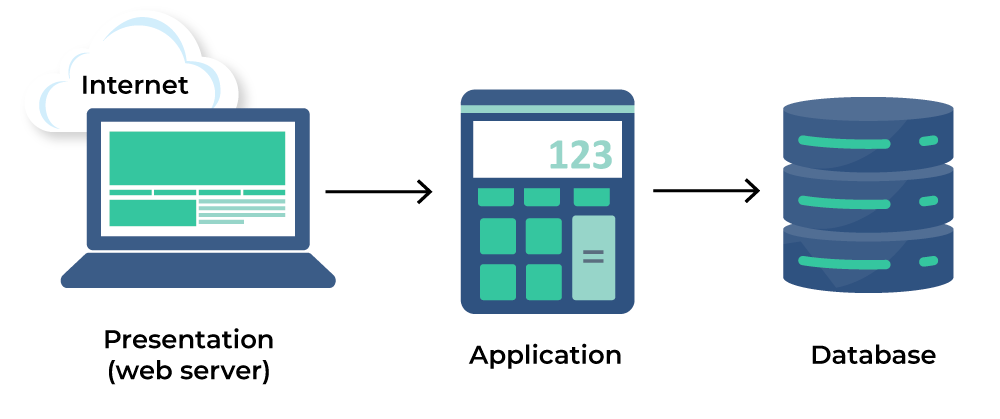
\includegraphics[width=1\textwidth]{Images/3-Tier-architecture.png}
\caption{\label{fig:3-tier}Schema di un'applicazione a tre livelli.}
\end{figure}

Il modello three-tier è un'architettura software\footnote{\glsdesc{software}} consolidata, di tipo client-server, in cui l'interfaccia utente, l'elaborazione logica e la gestione dei dati sono sviluppati e mantenuti come moduli indipendenti su server distinti. L'organizzazione in livelli separati aiuta a migliorare lo scopo dell'architettura stessa, aumentando quindi la manutenibilità, la scalabilità, l'affidabilità, la flessibilità e ovviamente la modularità del sistema.

Il maggior beneficio del modello three-tier è che i livelli sono sviluppati e mantenuti indipendentemente e perciò, in caso di qualsiasi modifica, solo un livello viene coinvolto. Inoltre, un ulteriore vantaggio è dato dal fatto che i livelli possono essere scalati separatamente, all'aumentare del carico di lavoro di uno qualsiasi.

Come si può intuire dal nome, il modello three-tier è composto da tre livelli: 
\begin{enumerate}
\item livello di presentazione
\item livello di applicazione
\item livello di \acrlong{db}
\end{enumerate}

% Nell'ambito dell'architettura three-tier, il termine `livello' viene spesso usato intercambiabilmente (sbagliando) al posto di `tier', come in `livello di presentazione' o `livello di logica di business', ma non sono la stessa cosa. 
% Un `livello' si riferisce ad una divisione funzionale del software, mentre un `tier' si riferisce a una divisione funzionale del software che viene eseguita su un'infrastruttura separata dalle altre divisioni. 
% Per esempio, l'applicazione `Contatti' sul telefono è un'applicazione a tre livelli, ma a singolo tier, perché tutti e tre i livelli vengono eseguiti sul telefono.
% La differenza è importante, perché i livelli non possono offrire gli stessi vantaggi dei tier.

Nello sviluppo web, i livelli hanno sempre i nomi precedenti, diversi gli uni dagli altri, ma si occupano di funzionalità analoghe.\newline

Nello specifico, il primo livello è quello che viene presentato all'utente finale, ossia l'interfaccia grafica grazie alla quale l'utente ha la possibilità di interagire con il sistema. Lo scopo principale dello strato superiore del modello three-tier è di mostrare le informazioni provenienti dagli altri livelli in modo chiaro e comprensibile all'utente e di raccogliere eventuali dati inseriti dall'utente stesso.
Il livello di presentazione può essere eseguito su un qualsiasi browser web, che farà anche da web server, su un'applicazione desktop o su un'interfaccia grafica \acrshort{gui}, a seconda delle esigenze del progetto.
Le applicazioni del livello di presentazione sono solitamente sviluppate utilizzando HTML, CSS e JavaScript, nel caso dei siti web, e possono essere scritte in un'ampia varietà di linguaggi a seconda della piattaforma, nel caso delle applicazioni desktop. Più di recente i \gls{framework} per lo sviluppo front-end, come \gls{angular}, React e Vue.js, sono diventati sempre più popolari. 

Nel caso di questo progetto di tirocinio, è stato scelto il \gls{framework} \gls{angular}, come verrà spiegato più approfonditamente nel seguito (\ref{sec:ang+prime}).\newline

Il secondo livello, quello di applicazione (o di logica) raccoglie informazioni e richieste dal livello superiore e le elabora utilizzando le regole specifiche della logica di business. Inoltre, il livello di applicazione può aggiungere, eliminare o modificare i dati memorizzati nel livello di \acrlong{db}; per esempio, nel caso di un e-commerce, il livello di applicazione fa query\footnote{\glsdesc{query}} al \acrlong{db} dell'inventario per sapere la disponibiltà di un prodotto, oppure aggiunge dettagli al profilo di un cliente, etc.
In breve, è il livello responsabile di processare le richieste del client e, una volta ricevute le informazioni necessarie, di inviarle di nuovo al client.
Nei sistemi più moderni o complessi, questo livello è solitamente sviluppato utilizzando linguaggi come Java, Python, PHP, Ruby, Perl, ASP.NET, \acrlong{js} o \acrlong{ts}, etc. In generale, qualsiasi linguaggio di programmazione che supporti le chiamate \gls{API}\footnote{\glsdesc{API}} (in modo da poter comunicare con il livello del \acrlong{db}, o con altri moduli) può essere utilizzato per sviluppare il livello di applicazione.\newline

Infine, nel terzo livello, quello di \acrlong{db}, detto anche livello di accesso ai dati o back-end, le informazioni elaborate dall'applicazione vengono archiviate e gestite, per poter essere recuperate in seguito, quando necessario. Il back-end si sostanzia in un \acrfull{dbms} e tra i più diffusi ricordiamo PostgreSQL, MySQL, MariaDB, Oracle, DB2, Informix, Microsoft SQL Server.\newline
% In alternativa, nei sistemi più moderni, si può utilizzare un \acrlong{db} NoSQL come Cassandra, CouchDB o MongoDB, ma questo è un argomento che esula dallo scopo di questo progetto di laurea.
% This layer is responsible for managing the data storage and retrieval in the system. It includes the database or file system where data is stored, as well as the data access layer (DAL) that interacts with the database to read and write data


----------------------------fermarsi qui e mettere solo una figura---------------------------\newline
I tre livelli sono collegati tra loro attraverso interfacce ben definite, che consentono a ciascun livello di funzionare in autonomia e una facile variazione e manutenzione dell'applicazione. L'architettura a tre livelli è un design pattern ampiamente utilizzato per la costruzione di applicazioni software scalabili e mantenibili e è comunemente utilizzato nelle applicazioni web e nei sistemi software aziendali.
% img

% Rules of the 3 Tier Architecture.
Si noti che il termine `3 Tier' non può essere riferito ad un'applicazione semplicemente dividendo il suo codice in tre parti. È fondamentale seguire determinate regole per ciascun livello in modo da garantire la corretta implementazione dell'architettura. Le suddette regole non sono complesse e di facile comprensione.
% letter list
\begin{itemize}
\item Innanzitutto, il codice di ogni livello deve essere memorizzato in file separati, i quali possono essere gestiti indipendentemente, meglio se da team diversi. Inoltre, ogni livello deve contenere solo il codice che appartiene a se stesso. Ciò significa che la logica di business deve risiedere soltanto nel livello di applicazione (logica di business), la logica di presentazione nel livello di front-end e la logica di accesso ai dati nel livello di back-end, o più precisamente nel livello di \acrfull{dal};
\item Il livello di presentazione può esclusivamente ricevere richieste da un'entità esterna e rispondere alla stessa, generalmente un utente, ma può anche essere un'altra applicazione software. In aggiunta, non può avere accesso diretto al \acrlong{db} o al livello di \acrlong{dal}, ma può unicamente inviare richieste e ricevere risposte dal livello contenente la logica di business (livello di applicazione);
\item Similmente, il livello di applicazione può solo ricevere richieste e rispondere al livello di presentazione, infatti, può solo inviare richieste e ricevere risposte dal \acrlong{dal} e gli è vietato di accedere direttamente al \acrlong{db};
\item Il \acrfull{dal} può ricevere richieste e rispondere solamente al livello della logica di business (applicazione) e non può inviare richieste a nessun altro componente, se non al \acrlong{dbms} che supporta;
\item È oltretutto importante assicurarsi che ogni livello sia totalmente ignaro del funzionamento interno degli altri. Ad esempio, il livello di applicazione deve essere agnostico rispetto al \acrlong{db} e non interessato al funzionamento interno dell'oggetto di accesso ai dati. Allo stesso modo, non deve elaborare i dati in modo diverso in base al componente che riceve una richiesta. Il livello di presentazione può prendere i dati e elaborarli in vari modi, come ad esempio costruire un documento HTML, un documento PDF, un file CSV, ma sono dettagli non dovrebbero influenzare il livello di applicazione.
\end{itemize}


Si noti che, in un'applicazione a tre livelli, tutte le comunicazioni passano attraverso il livello applicazione. Il livello di presentazione e il livello di \acrlong{db} non possono comunicare direttamente tra loro.

Di nuovo, il principale beneficio dell'architettura a tre livelli è la separazione logica delle funzionalità. Ogni livello può essere eseguito su un sistema operativo e una piattaforma server diversi, ad esempio un livello di presentazione può essere eseguito su un server web, mentre il livello di applicazione può essere eseguito su un server di applicazioni e il livello di \acrlong{db} può essere eseguito su un server \acrlong{db}; per far si che ognuno combaci coi propri requisiti funzionali e che ogni livello sia eseguito su un server dedicato (fisico o virtuale), cosicché i servizi di ciascun livello possano essere personalizzati e ottimizzati senza influenzare gli altri livelli.

Altri vantaggi includono:
\begin{itemize}
\item Sviluppo più rapido: poiché ogni livello può essere sviluppato simultaneamente da team diversi, un'organizzazione può portare l'applicazione sul mercato più rapidamente e i programmatori possono utilizzare i linguaggi e gli strumenti più recenti e migliori per ogni singolo livello;
\item Miglior scalabilità: ogni livello può essere scalato indipendentemente dagli altri, se necessario;
\item Miglior affidabilità: un'interruzione (di corrente o per un problema software) in un livello è meno probabile che influenzi la disponibilità o le prestazioni degli altri livelli;
\item Miglior sicurezza: poiché il livello di presentazione e il livello di \acrlong{db} non possono comunicare direttamente tra loro, un livello di applicazione ben progettato può funzionare come una sorta di firewall interno, prevenendo attacchi come le SQL injection o altri exploit dannosi.
\end{itemize}


Si noti che esistono altre tipologie di architetture software multi-tier, come ad esempio quella a due livelli, la N-tier, il \acrshort{mvc}, etc, ma non sono così diffuse come quella a tre livelli e non saranno approfondite in questo progetto di laurea.\newline
---------------------------------------------------------------------------------------------

Un paragone degno di nota è quello con il \acrfull{mvc}. Le principali \textbf{differenze} tra le architetture di tipo three-tier e di tipo \acrshort{mvc} sono:
\newline\newline oppure\newline

L'architettura a tre livelli sembra molto simile a un'altra architettura, altrettanto conosciuta, denominata \acrfull{mvc}, ma non sono la stessa cosa.

Entrambe le architetture mirano a separare i compiti dell'applicazione e a migliorare lo sviluppo del software suddividendola in diversi componenti.
Mentre l'architettura a tre livelli -come visto in precedenza (\ref{sec:3-tier})- si concentra sul dividere un'applicazione in tre livelli distinti (ogni livello ha il suo ruolo specifico) e sulla comunicazione ben definita tra di loro (come descritto nelle regole), l'architettura \acrshort{mvc}, tuttavia, si concentra sulla separazione dell'applicazione in tre componenti distinti: Model, View e Controller (modello, vista e controllore).

Il modello rappresenta i dati e la logica di business dell'applicazione, la vista rappresenta l'interfaccia utente e il controllore agisce come mediatore tra i primi due. Infatti, è il controllore a ricevere l'input\footnote{\glsdesc{input}} dall'utente, a interagire con il modello per elaborare i dati e ad aggiornare la vista per visualizzarne i risultati.

In breve, entrambe cercano di separare le responsabilità e migliorare lo sviluppo del software, ma lo portano a termine diversamente: 
\begin{itemize}
    \item il modello three-tier si concentra di più sulla separazione dei diversi livelli;
    \item l'architettura \acrshort{mvc} si concentra di più sulla separazione dei componenti all'interno di un livello.
\end{itemize}

\begin{figure}[H]
\centering
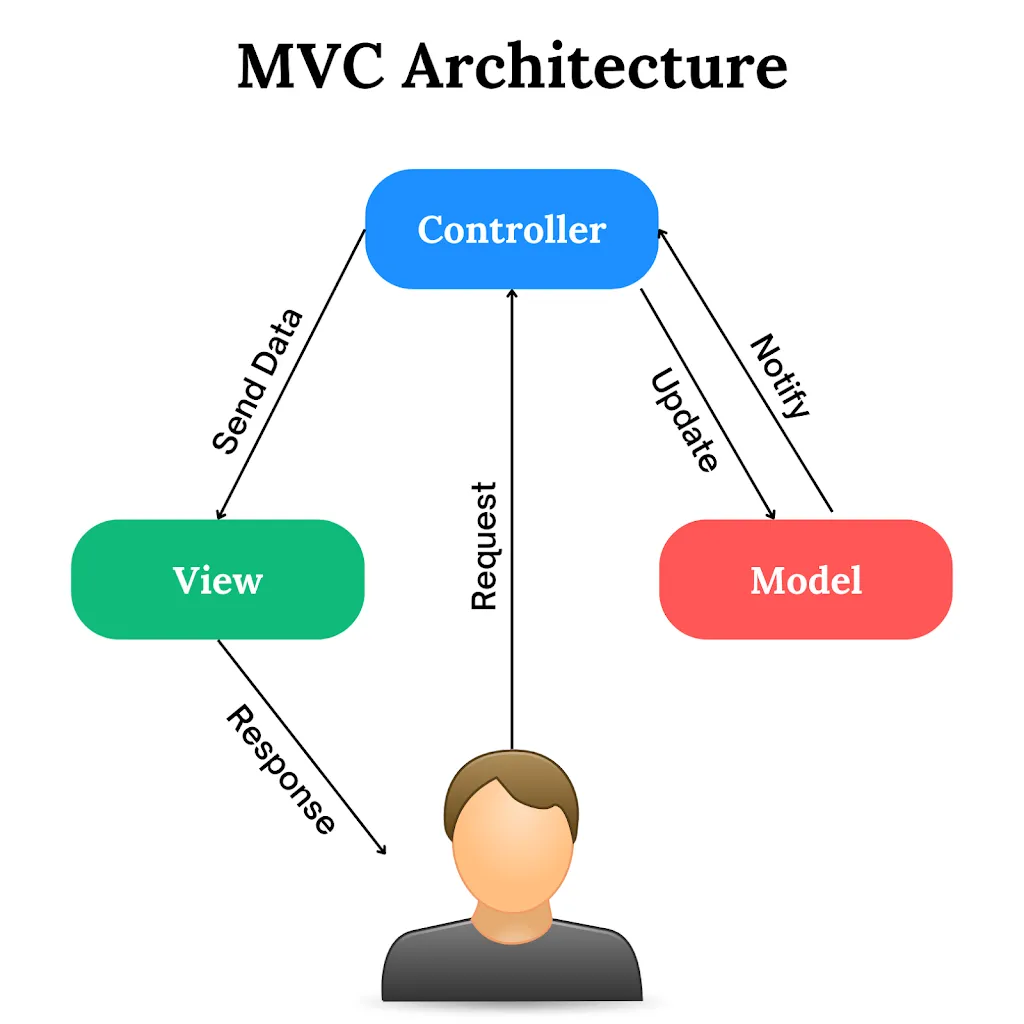
\includegraphics[width=1\textwidth]{Images/mvc.png}
\caption{\label{fig:mvc}Schema teorico dell'architettura \acrshort{mvc}.}
\end{figure}

\begin{figure}[H]
\centering
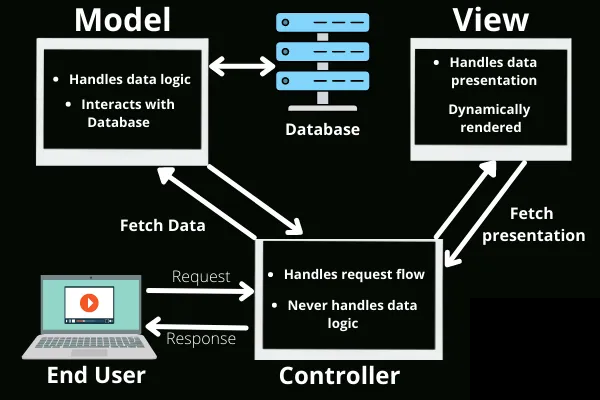
\includegraphics[width=1\textwidth]{Images/model-view-controller.png}
\caption{\label{fig:mvc2}Schema pratico dell'architettura \acrshort{mvc}.}
\end{figure}


\newpage
\section{Framework utilizzati}\label{sec:Framework}
\begin{figure}[H]
\centering
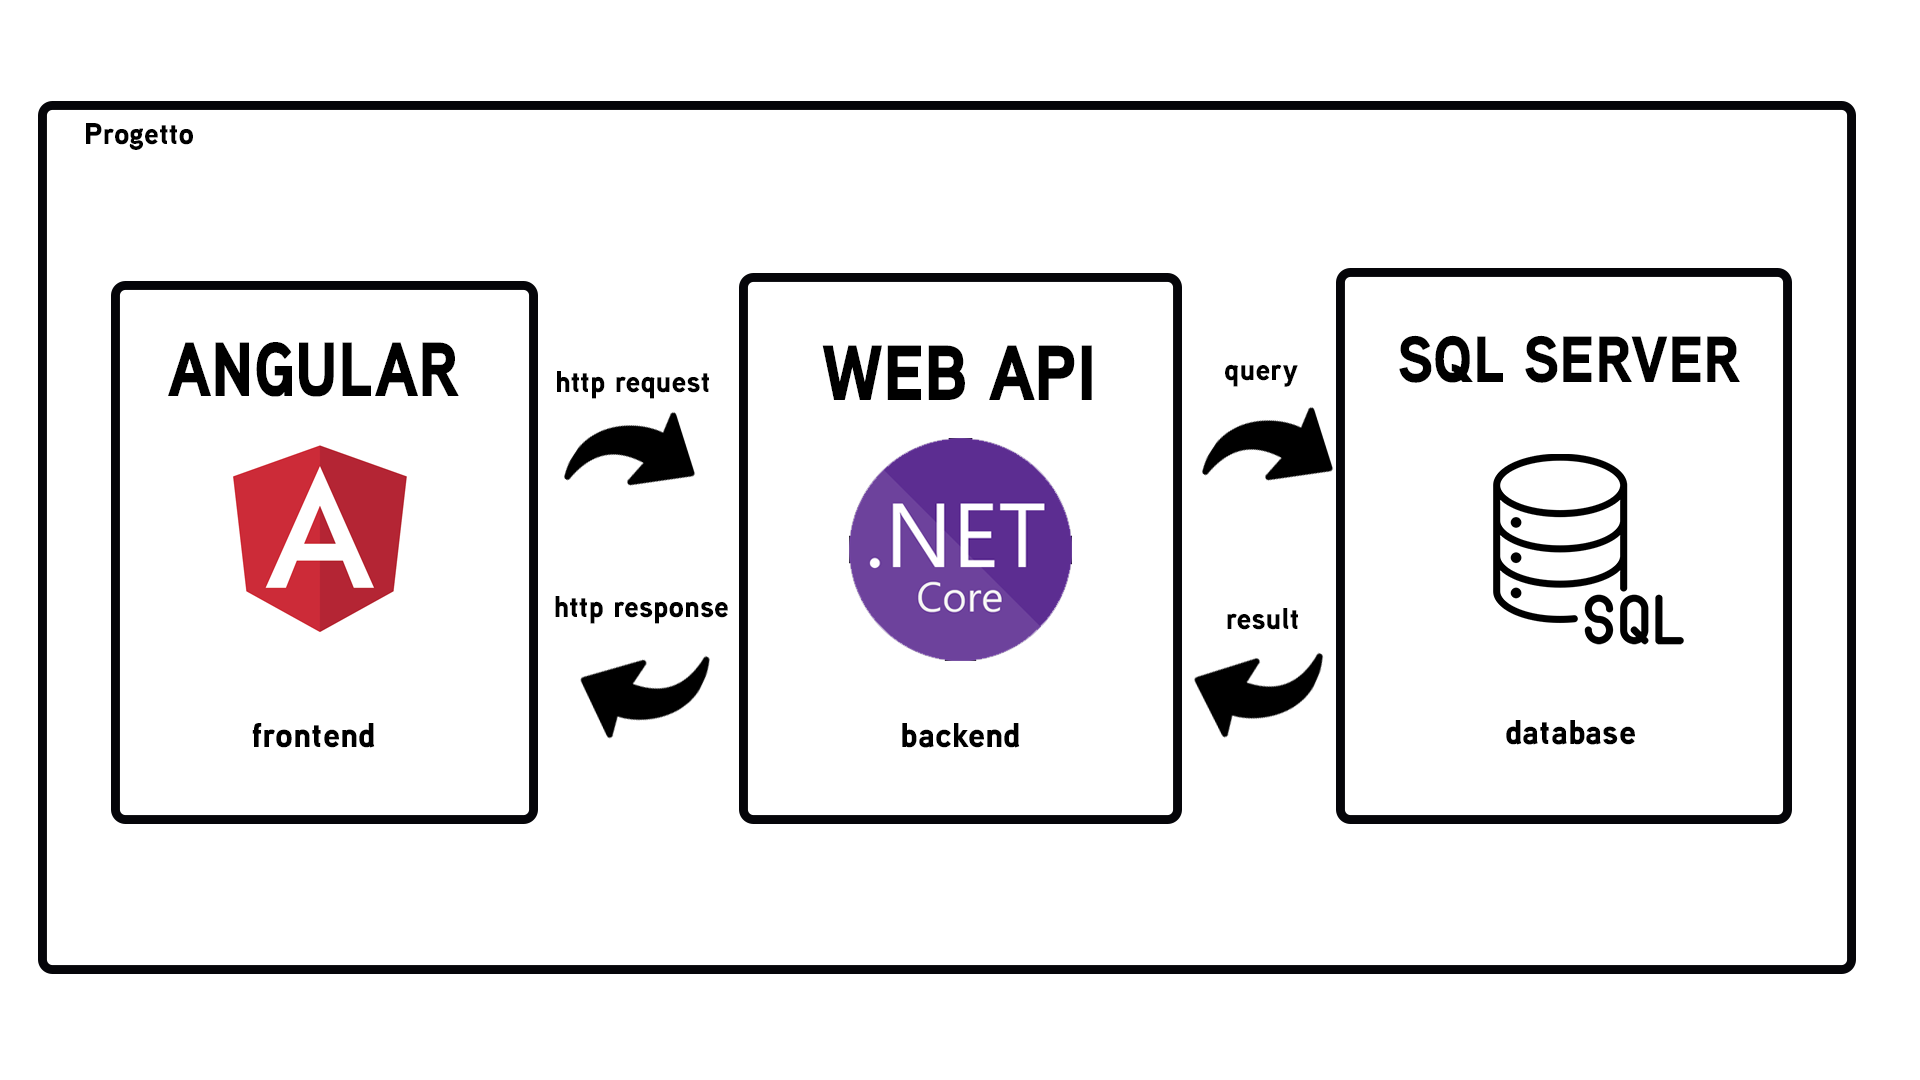
\includegraphics[width=1\textwidth]{Images/architettura.png}
\caption{\label{fig:arch}Schema dei \gls{framework} utilizzati.}
\end{figure}
Dopo aver esaminato l'architettura del modello three-tier, in questa sezione verranno descritti i \gls{framework} utilizzati per lo sviluppo del progetto di laurea.\newline

Un \gls{framework} è un'astrazione che unisce codice comune tra progetti di software con scopi simili, fornendo una funzionalità generale, che può essere modificata o estesa per risolvere un problema specifico.
Più in generale, incrementano l'efficienza e le prestazioni dello sviluppo web, fornendo una struttura coerente, affinché gli sviluppatori non debbano continuamente ricostruire il codice da zero; i \gls{framework} sono ottimi quando si tratta di risparmiare tempo. 

Aggiuntivamente, offrono ai programmatori una serie di funzionalità extra che possono essere aggiunte al \acrlong{sw} senza richiedere ulteriori sforzi.\newline

Nel caso di questo progetto di laurea, lo scopo principale è stato quello di implementare nuovi componenti e funzionalità per un'applicazione web già esistente, quindi è stato necessario utilizzare i \gls{framework} già adottati nel progetto stesso, in modo da poter integrare le nuove funzionalità in uno dei modi più semplici e veloci, senza dover riscrivere totalmente il codice da zero. Uno dei difetti di questo approccio è stato aver ricevuto del software scritto da più sviluppatori, con stili di programmazione diversi e componenti sviluppati da una o più persone. Infatti la repository del progetto (dopo aver implementato le funzionalità richieste dal progetto di laurea) è composta da più di 55 mila file e nel complesso era molto facile perdersi nella moltitudine di file.
Ciononostante, è stato possibile integrare le nuove funzionalità in modo semplice e veloce, grazie ai \gls{framework} di sviluppo utilizzati, sia per il back-end che per il front-end.

\subsection{Angular e PrimeNG}\label{sec:ang+prime}
\begin{figure}[H]
\centering

\includegraphics[width=.5\textwidth]{Images/ang+prime.png}
\caption{\label{fig:ang+prime}Angular e PrimeNG, due \gls{framework}.}
\end{figure}
Questa sotto-sezione si propone di descrivere e analizzare in breve uno dei \gls{framework} per il front-end più utilizzati al mondo, \gls{angular}, insieme al relativo \gls{framework} -\gls{open source}\footnote{\glsdesc{open source}}- \acrshort{primeng}, che fornisce uno dei set di componenti \acrshort{ui} più completi per \gls{angular}.\newline

\gls{angular}, denominato anche \gls{angular} 2+ (ossia una versione più moderna di \gls{angularjs}), è un \gls{framework} \acrlong{js} scritto e basato su \acrlong{ts}, open source per lo sviluppo di \acrshort{ui} di applicazioni web, focalizzandosi sulle singole pagine; è stato sviluppato principalmente dal team di \gls{angular} di Google e da una comunità di individui e aziende esterne. È, inoltre, una riscrittura completa del \gls{framework} originale (AngularJS); entrambi i \gls{framework} sono stati sviluppati dallo stesso team. Attualmente, \gls{angular} è mantenuto da Google.

Le differenze principali tra \gls{angular} e \gls{angularjs} sono che il secondo usa \acrlong{js}, ha un supporto mobile limitato e una dependency injection meno robusta. Il primo invece (\gls{angular}) invece adotta \acrlong{ts}, offre un supporto mobile migliore, una dependency injection più potente e un efficiente rilevamento dei cambiamenti. Inoltre, ha template\footnote{\glsdesc{template}} dinamici, una \acrshort{cli} potente e una struttura modulare per file più piccoli.\newline

In quanto \gls{framework}, fornendo una struttura standard per gli sviluppatori, \gls{angular} ha dei chiari vantaggi. Consente agli utenti di creare applicazioni di grandi dimensioni, manutenibilmente.  

% Differences between Angular and AngularJS
    % Google designed Angular as a ground-up rewrite of AngularJS.

    % Angular does not have a concept of "scope" or controllers; instead, it uses a hierarchy of components as its primary architectural characteristic.[5]
    % Angular has a different expression syntax, focusing on "[ ]" for property binding, and "( )" for event binding[6]
    % Modularity – much core functionality has moved to modules
    % Angular recommends the use of Microsoft's TypeScript language, which introduces the following features:
    % Static typing, including Generics
    % Type annotations
    % Dynamic loading
    % Asynchronous template compilations
    % Iterative callbacks provided by RxJS.
    % Support to run Angular applications on servers.
%

La principale funzionalità di \gls{angular} è quella di fornire blocchi per costruire le applicazioni web, denominati componenti, grazie ai quali aiuta gli sviluppatori ad impostare rapidamente una web-app scalabile e facilmente manutenibile. 
\gls{angular} conferisce ai programmatori la libertà di sviluppare applicazioni che possano essere eseguite agilmente su più piattaforme; inclusi dispositivi mobili, desktop e web. Oltretutto, è stato progettato per essere modulare, cosicché si possano integrare o rimuovere facilmente le funzionalità di cui si ha bisogno o meno.

Nonostante l'ampio utilizzo e la facilità di apprendimento di \acrlong{js}, nei casi analoghi a questo progetto di laurea, \gls{angular} si rivela comunque essere una scelta migliore, presentando una serie di benefici -sopra citati i principali- che lo rendono ideale per affrontare la maggior parte, se non tutti, i problemi che gli sviluppatori incontrano con \acrlong{js}. 

Alcune delle caratteristiche di \gls{angular} sono:
\begin{enumerate}
    \item \acrfull{dom}: gestisce un documento \acrshort{xml} o \acrshort{html} come una struttura ad albero in memoria; \gls{angular} usa il \acrshort{dom} classico. Ipotizzando che vengano effettuati dieci aggiornamenti sulla stessa pagina \acrshort{html}, invece di aggiornare i cambiamenti già elaborati, \gls{angular} aggiorna l'intera struttura ad albero dei tag \acrshort{html};
    \item \acrfull{ts}: il linguaggio -sviluppato da Microsoft- in cui è scritto \gls{angular}. Definisce un insieme di tipi che rende il codice più facile da leggere e da scrivere. Inoltre, tutto il codice \acrlong{ts} viene compilato in \acrlong{js}, cossicché ogni piattaforma possa eseguirlo. È altamente consigliato, ma non vincolante per sviluppare con \gls{angular};
    \item Data Binding: è un meccanismo che abilita gli utenti a manipolare gli elementi di una pagina web attraverso un browser web. Usato principalmente nelle pagine web che incorporano componenti interattivi, come calcolatori, tutorial, forum e giochi. Inoltre, consente una migliore visualizzazione progressiva di una pagina web quando le pagine contengono una grande quantità di dati. Nel caso di \gls{angular} viene utilizzato data binding bidirezionale, infatti lo stato del modello riflette eventuali modifiche apportate agli elementi \acrshort{ui} corrispondenti. Al contrario, lo stato \acrshort{ui} riflette eventuali modifiche apportate allo stato del modello, questa funzionalità consente al \gls{framework} di collegare il \acrshort{dom} ai dati del modello attraverso il controller;
    \item Tesing: \gls{angular} usa un test \gls{framework} denominato Jasmine, ma non sarà oggetto di discussione in questo progetto di laurea;
\end{enumerate}

Passando all'architettura, è importante notare che \gls{angular} è un \gls{framework} \acrlong{mvc}, a tutti gli effetti, dando una guida chiara su la web app dovrebbe essere strutturata; permette inoltre un flusso bidirezionale di data-binding mettendo contemporaneamente a disposizione un vero e proprio \acrshort{dom}.

I seguenti sei sono i blocchi fondamentali di un'applicazione \gls{angular}:
\begin{enumerate}
    \item Moduli: una web app \gls{angular} possiede un modulo root (denominato AppModule) il quale fornisce il meccanismo di bootstrap per avviare l'applicazione. Ogni modulo può avere uno o più moduli figlio;
    \item Componenti: ogni componente dell'applicazione definisce una classe che contiene i dati e la logica dell'applicazione. Generalmente, un componente definisce una parte dell'interfaccia grafica (o \acrshort{ui}, in inglese);
    \item Modelli (o Template\footnote{\glsdesc{template}}): i template \gls{angular} combaciano con \acrshort{html} per modificare i suoi stessi elementi (\acrshort{html}) prima che sia visualizzati. Esistono due tipi di data binding: di evento (bisogna aggiornare la web app) e di proprietà (abilita l'utente ad interpolare i valori calcolati dall'applicazione nel codice \acrshort{html});
    \item Metadati: comunicano ad \gls{angular} come processare una classe. Sono usati per decorare la classe stessa, cosicché si possa configurare il comportamento aspettato della classe;
    \item Servizi: una classe di servizio è creata quando si hanno dati o logica che non sono associati con la visualizzazione, ma devono comunque essere condivisi tra i componenti. La classe di servizio è sempre associata con il decoratore `@Injectable';
    \item Dependency Injection: un pattern di progettazione che permette di mantenere le classi dei componenti precise e efficienti. È una funzionalità che non raccoglie dati da un server, valida un input dell'utente o stampa direttamente a console. Invece, delega i suddetti compiti ai servizi;
\end{enumerate}

\begin{figure}[H]
\centering
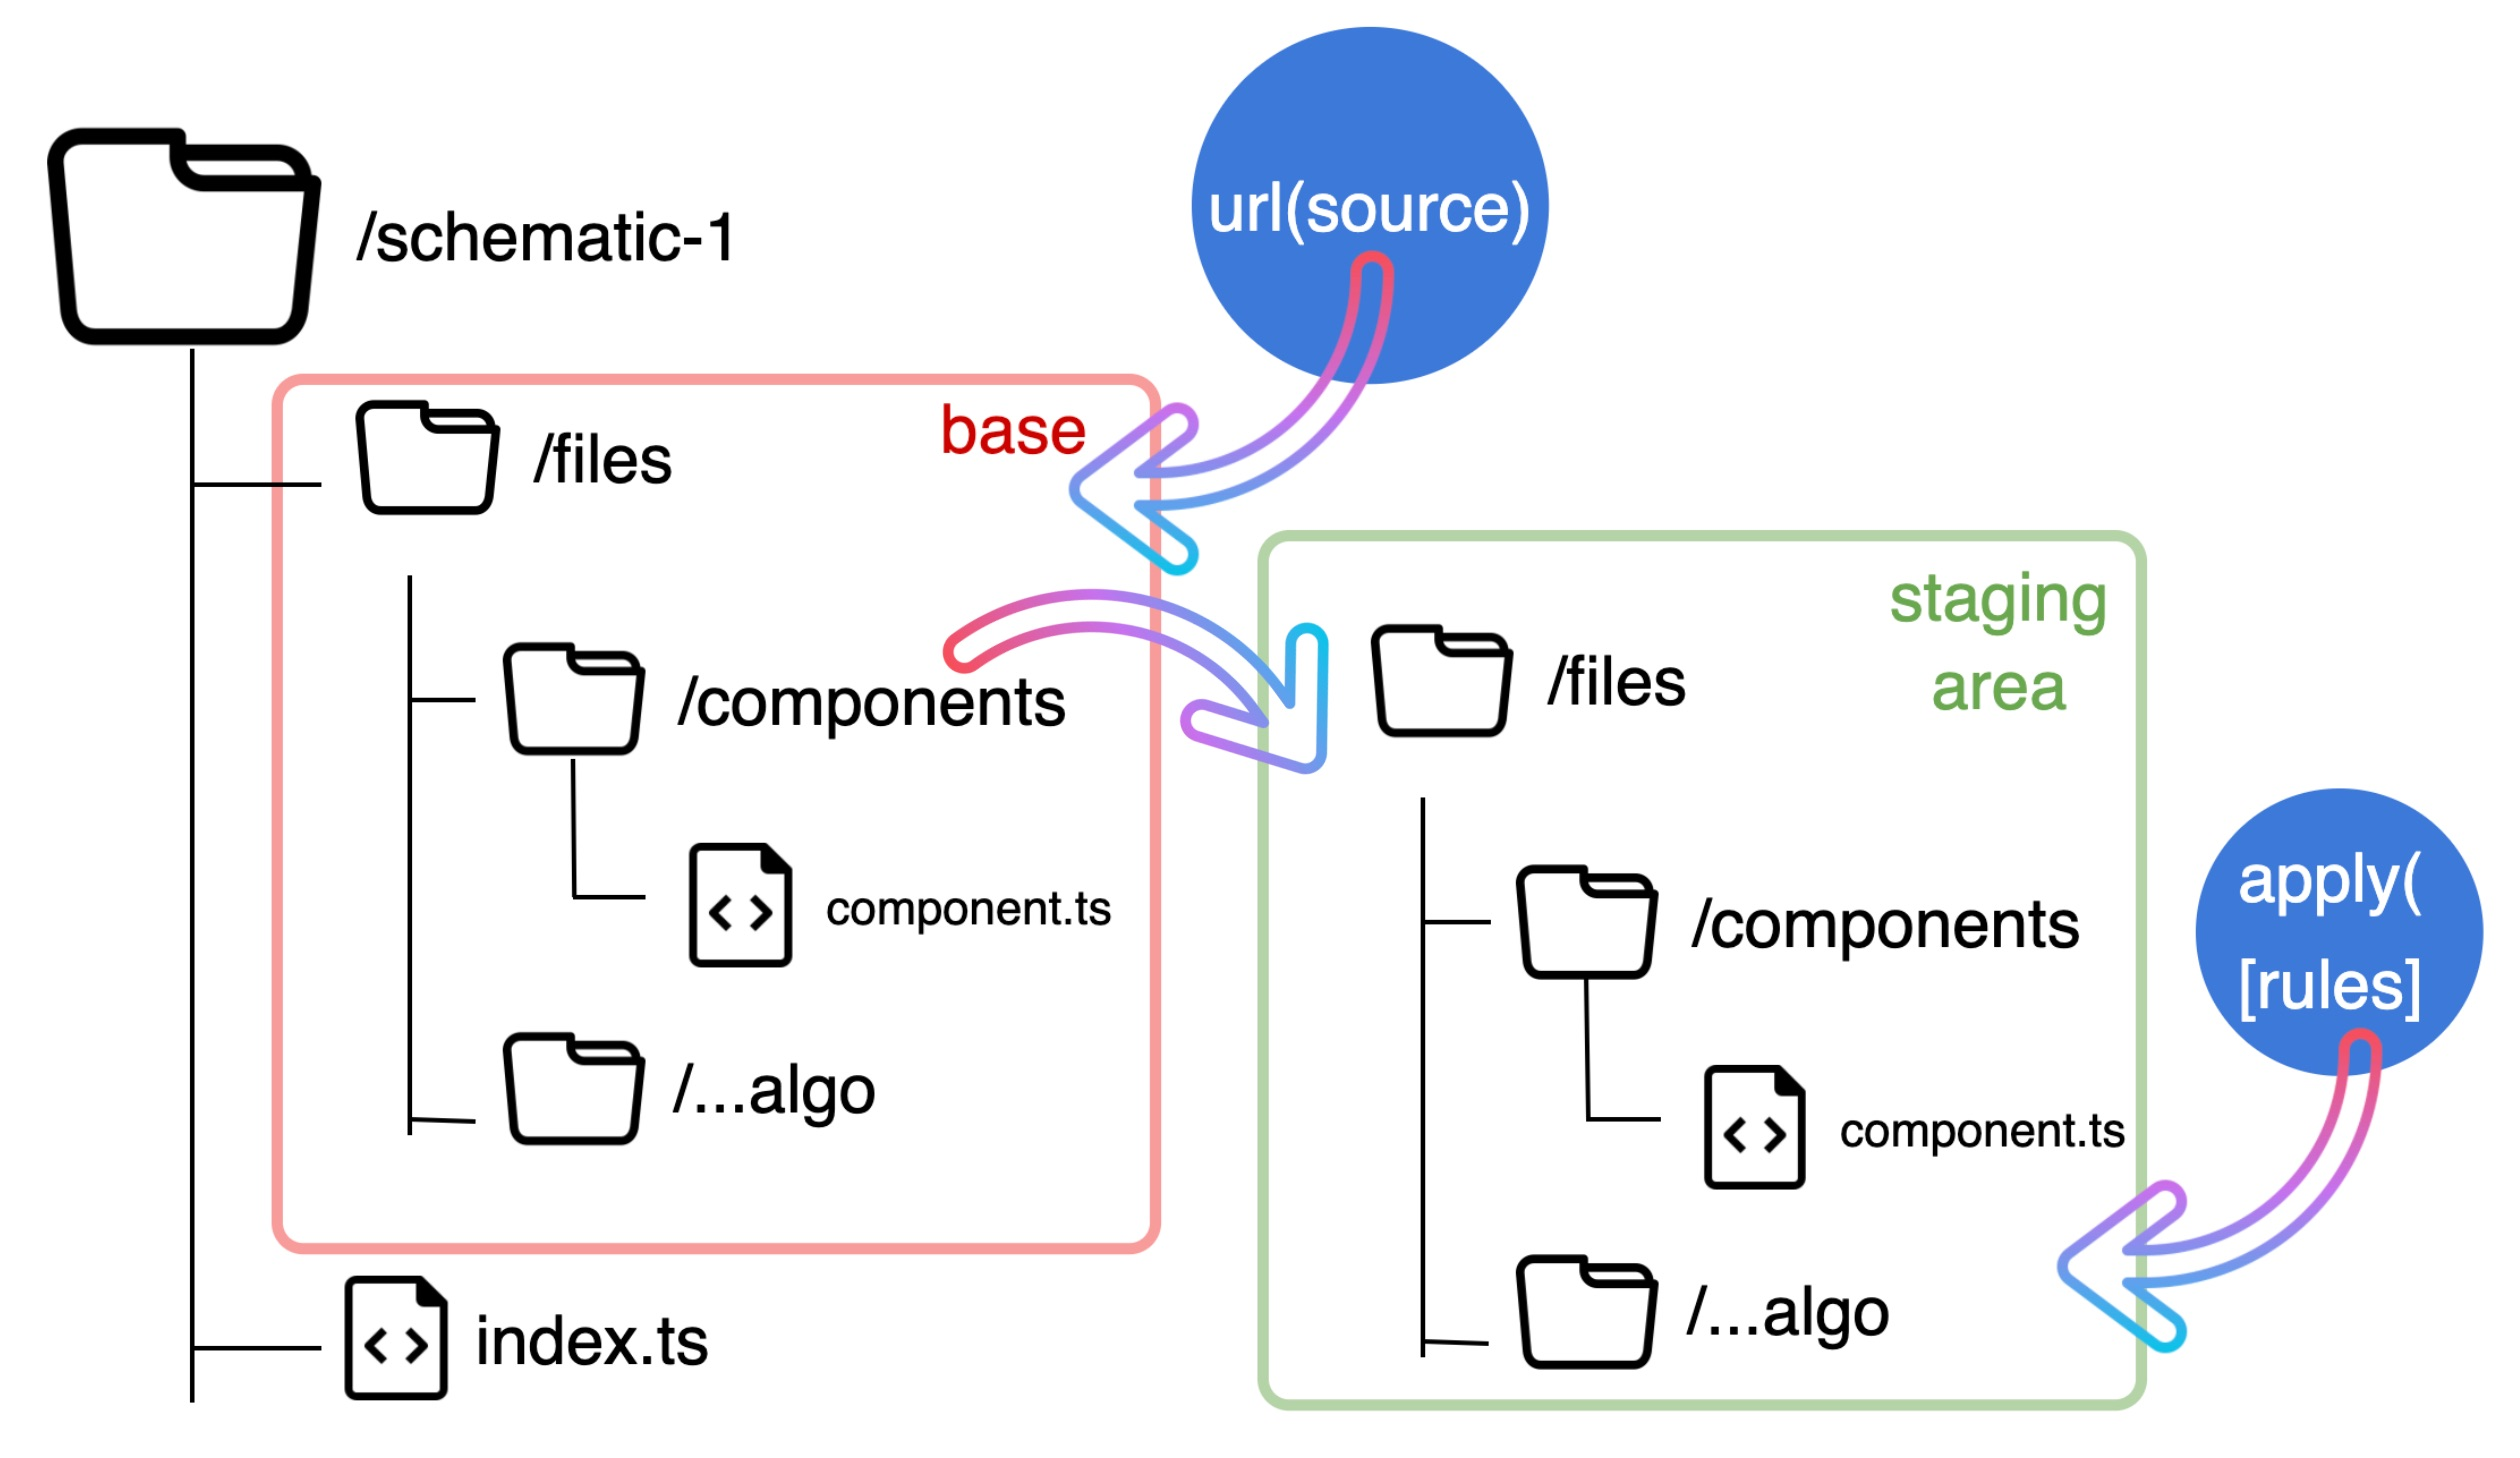
\includegraphics[width=1\textwidth]{Images/schematic angular.jpg}
\caption{\label{fig:angular schematic}Schematica di Angular.}
\end{figure}


Un'ulteriore funzionalità degna di nota di \gls{angular} è la sua \acrfull{cli}, la quale permette di creare nuovi progetti, applicazioni, componenti, etc. Inoltre, \gls{angular} \acrshort{cli} offre anche la possibilità di eseguire un web server, tramite l'apposoto comando da terminale, in modo tale da poter testare l'applicazione in locale, prima di effettuare il \gls{deploy} su un server remoto.\newline

% \subsection{Angular advantages}\label{sec:Angular-advantages}
Molte versioni di \gls{angular} sono state rilasciate dalla sua nascita. Ognuna di esse ha contribuito al miglioramento dell'efficienza del \gls{framework}.
I principali \textbf{vantaggi} di \gls{angular} sono:

\begin{enumerate}
    \item Componenti su misura: funzionalità che permette agli utenti di creare i propri componenti, i quali possono contenere funzionalità e logiche di visualizzazione in parti riutilizzabili. Inoltre si integrano facilmente con i componenti \acrshort{html} standard;
    \item Data Binding: funzionalità che permette agli utenti di trasformare i dati da codice \acrshort{js} a \acrshort{ui} agevolmente, senza dover scrivere codice aggiuntivo;
    \item Dependency Injection\footnote{\glsdesc{Dependency Injection}}: funzionalità che permette agli utenti di creare servizi modulari e `iniettarli' dove necessario. Migliora la modularità e la manutenibilità degli stessi servizi;
    \item Testing: i test sono utensili di prima classe, \gls{angular} è stato sviluppato da zero tenendolo a mente, infatti permette di testare ogni singola parte dell'applicazione;
    \item Esaustivo: fornisce soluzioni per la comunicazione coi server, l'instradamento nell'applicazione e altro tra le funzionalità standard;
    \item Compatibilità: \gls{angular} è utilizzabile su più piattaforme e compatibile con vari browser. Un'applicazione \gls{angular} può essere eseguita su qualsiasi browser (Chrome, Firefox, Safari, etc) o sistema operativo (Windows, Linux, MacOS, etc).
\end{enumerate}

\begin{figure}[H]
\centering
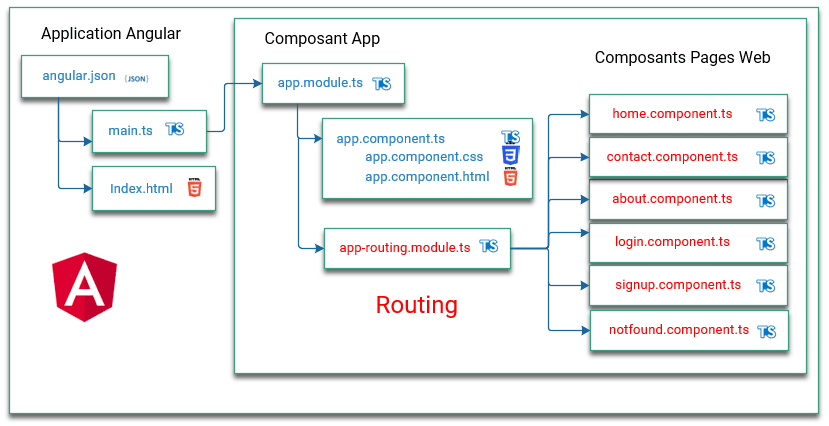
\includegraphics[width=1\textwidth]{Images/routing-architecture-angular.png}
\caption{\label{fig:angular routing}Schema dell'instrademento di Angular.}
\end{figure}

I principali \textbf{svantaggi} e limitazioni di \gls{angular} sono:

\begin{enumerate}
    \item Curva di apprendimento ripida: i componenti elementari di \gls{angular} che tutti i sviluppatori dovrebbero conoscere comprendono direttive, moduli, decoratori, componenti, servizi, dependency injection, pipe e template. Alcuni argomenti più avanzati includono rilevamento di cambiamenti, zone, compilazione \acrshort{aot}\footnote{\glsdesc{Ahead-of-Time}} e \acrshort{rxjs}. Per i neofiti, \gls{angular} potrebbe essere impegnativo da apprendere per via della sua completezza;
    \item \acrshort{seo} limitate: \acrshort{seo} limitate e scarsa accessibilità all'indicizzazione\footnote{\glsdesc{SEO}} dei motori di ricerca;
    \item Migrazione: una delle ragioni per cui le aziende non adottano frequentemente \gls{angular} per le migrazioni è la difficoltà intrinseca nella portabilità di codice \acrshort{js} (o basato su \gls{jquery}\footnote{\glsdesc{jquery}}) preesistente in un'applicazione \gls{angular}. Inoltre, ogni nuova versione rischia di essere problematica da aggiornare e molte di loro non sono retro-compatibili.
    \item Verboso: un problema comune negli utilizzatori \gls{angular} è la verbosità del \gls{framework}.
\end{enumerate}

Tra le aziende più famose che utilizzano \gls{angular} ci sono Google, Microsoft, Nike, Forbes, Upwork, HBO, Sony, General Motors, etc.

\newpage % parte di PrimeNG
Infine, \textbf{\acrfull{primeng}} è una collezione ricca di componenti \acrshort{ui} per \gls{angular}, i cui widget sono \gls{open source} e gratuiti. Sviluppato da PrimeTek Informatics nel 2016, un'azienda con anni di esperienza nello sviluppo di soluzioni \acrshort{ui} \gls{open source}.

Tra le varie funzionalità che rendono \acrshort{primeng} un \gls{framework} popolare tra gli sviluppatori, ci sono:
\begin{itemize}
% \item \textbf{Rich UI Components:} testo in grassetto :)
\item Componenti \acrshort{ui} completi: \acrshort{primeng} offre oltre 80 componenti \acrshort{ui}, come ad esempio tabelle, dialoghi, grafici, etc;
\item Template-Driven\footnote{\glsdesc{template-driven}}: i componenti di \acrshort{primeng} sono template-driven, rendendoli facili da usare e personalizzare;
\item Supporto di temi: \acrshort{primeng} supporta vari temi, permettendo agli sviluppatori di scegliere tra una vasta gamma.
\end{itemize}

\begin{figure}[H]
\centering
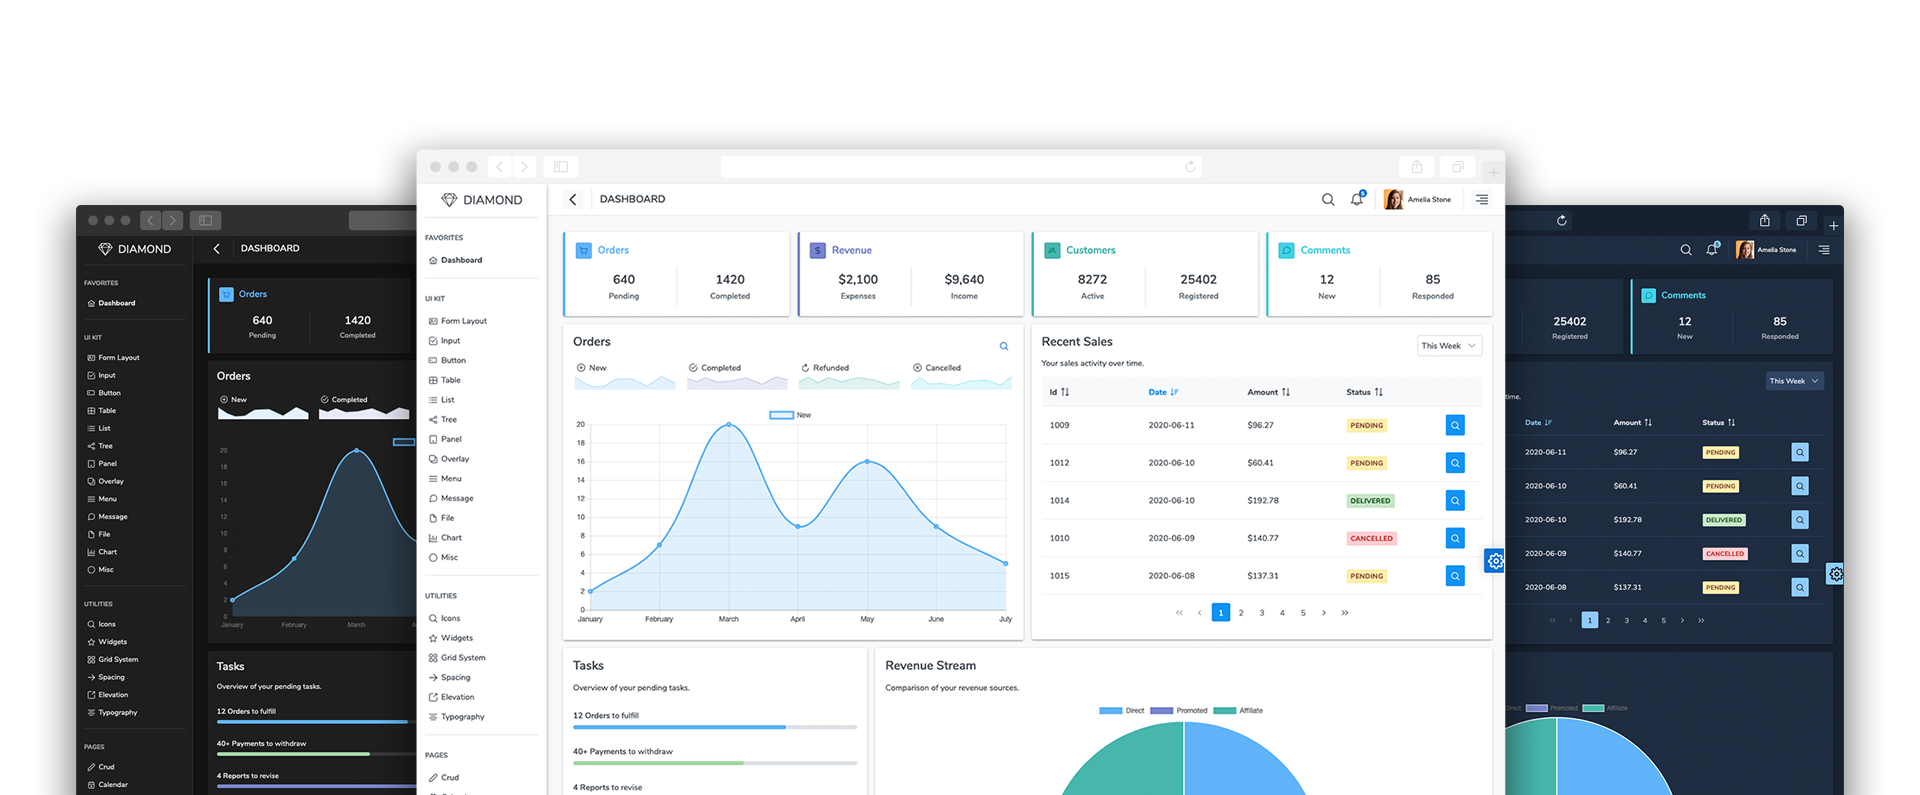
\includegraphics[width=1\textwidth]{Images/diamond.png}
\caption{\label{fig:diamond}Diamond, uno dei template di PrimeNG.}
\end{figure}

Parecchie aziende usano \acrshort{primeng} sia per applicazioni interne che per applicazioni per i clienti. Grazie alla sua numerosa serie di componenti e facilità d'uso, \acrshort{primeng} è diventato una delle scelte più popolari e valide tra gli sviluppatori, anche per le applicazioni più complesse.\newline
Tra di loro troviamo Ericsson, Siemens, Lufthansa, UniCredit, Ford, Volvo, Nvidia, eBay, Mercedes-Benz, Audi, HP, Scania, Cisco, Nike, Wolkswagen.

\begin{figure}[H]
\centering
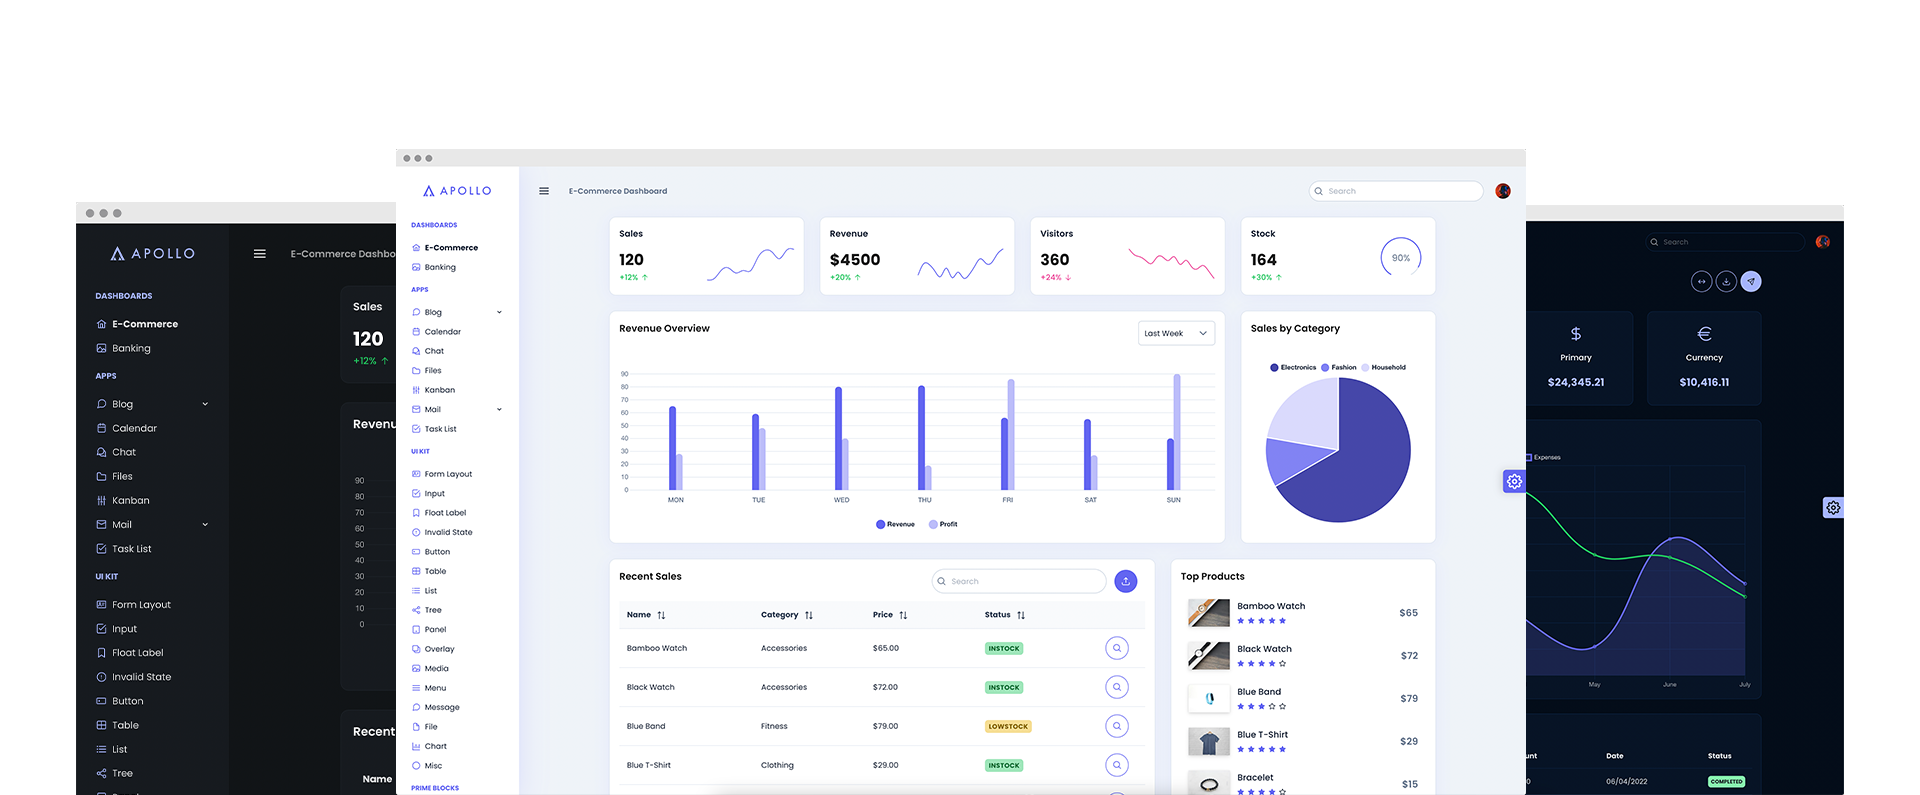
\includegraphics[width=1\textwidth]{Images/apollo.png}
\caption{\label{fig:apollo}Apollo, uno dei template di PrimeNG.}
\end{figure}
\begin{figure}[H]
\centering
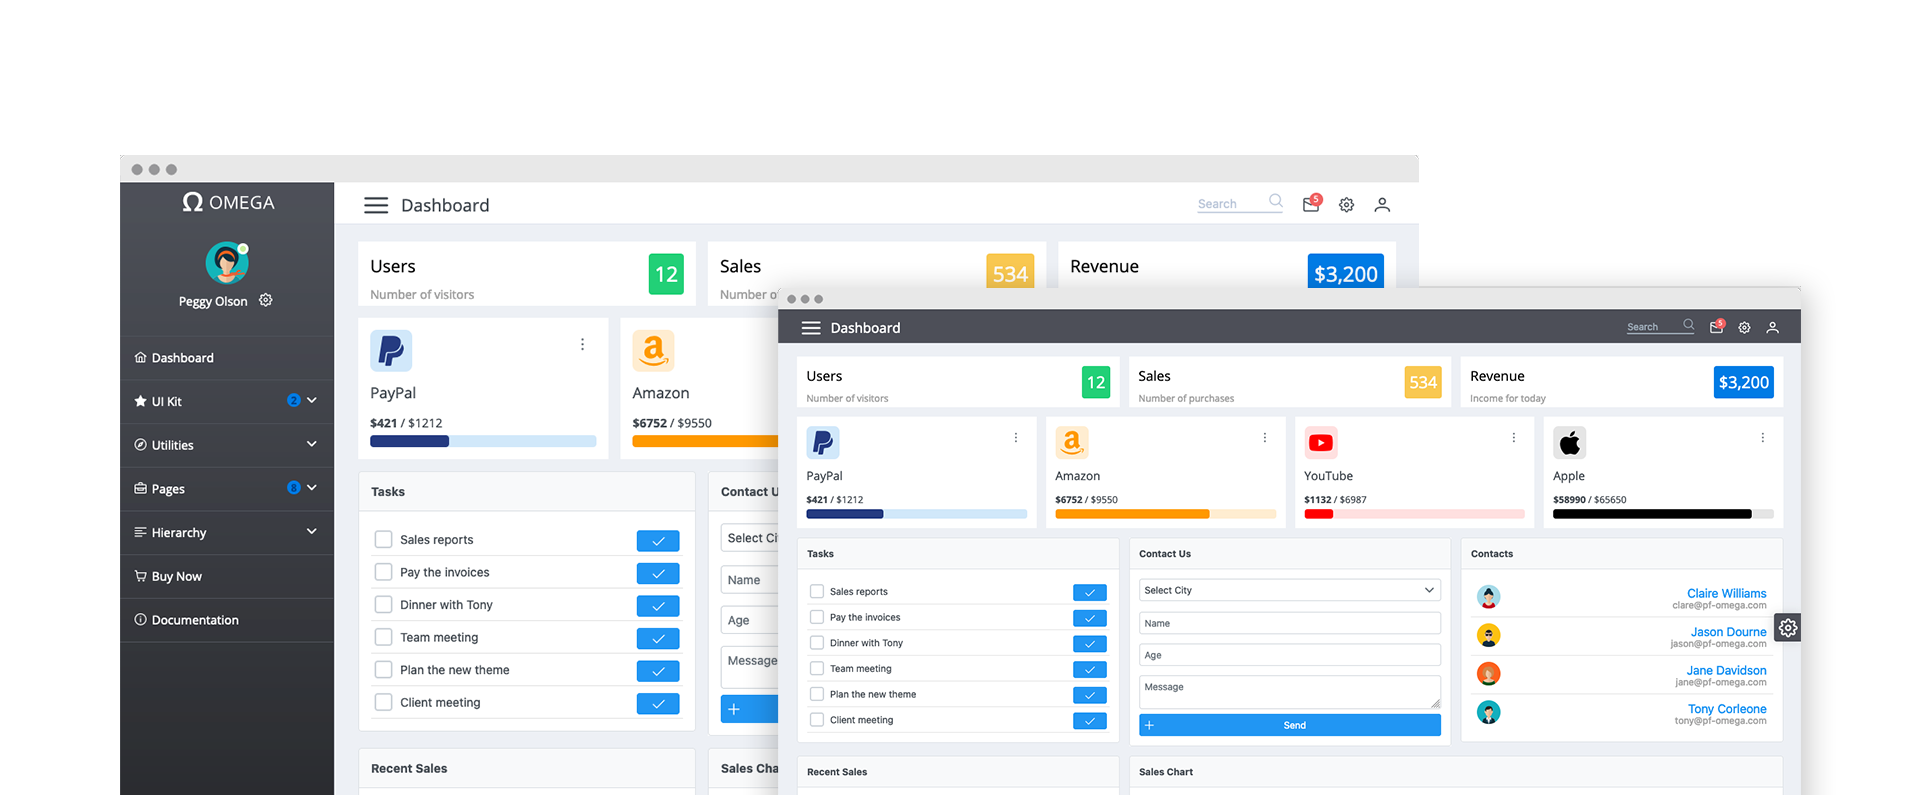
\includegraphics[width=1\textwidth]{Images/omega.png}
\caption{\label{fig:omega}Omega, uno dei template di PrimeNG.}
\end{figure}

\newpage
\subsection{Typescript}\label{sec:Typescript}
\begin{figure}[H]
\centering

\includegraphics[width=.7\textwidth]{Images/ts.png}
\caption{\label{fig:logo ts}Il logo di TypeScript.}
\end{figure}
\acrfull{ts} è un linguaggio di programmazione \gls{open source} sviluppato e mantenuto da Microsoft. Fa parte di un approccio moderno alla programmazione e è un superset sintattico e restrittivo di \acrlong{js}, infatti offre tutte le funzionalità di \acrlong{js} e ne aggiunge di nuove e più avanzate, come la possibilità di tipare staticamente il linguaggio. In particolare, siccome \acrlong{ts} `conosce' il linguaggio \acrlong{js}, in molti casi genererà i tipi inferenziandoli\footnote{\glsdesc{inferenza}} dal codice. Per esempio, inizializzando una variabile con un valore arbitrario, \acrlong{ts} userà il valore come tipo. 

\begin{figure}[H]
\centering
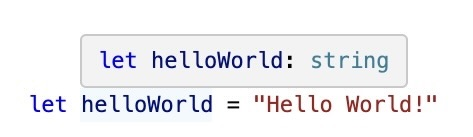
\includegraphics[width=.8\textwidth]{Images/ts hello.jpg}
\caption{\label{fig:hello}Inizializzazione del classico `Ciao Mondo'.}
\end{figure}

Comprendendo come funziona \acrlong{js}, \acrlong{ts} può costruire un sistema di tipi che accetta il codice \acrlong{js}, ma coi tipi; ciò offre un sistema di tipi completo, senza dover aggiungere caratteri extra per renderli espliciti. Infatti, è così che \acrlong{ts} è in grado di capire che `helloWorld' è una stringa nell'esempio sopra, nella figura (\ref{fig:hello}).
Visual Studio Code, sviluppato da Microsoft e uno dei text editor più popolari tra gli sviluppatori, usa \acrlong{ts} per facilitare l'esperienza della scrittura del codice. 

Inoltre, \acrlong{ts} è stato progettato per lo sviluppo di applicazioni di grandi dimensioni e viene transcompilato\footnote{\glsdesc{transcompilare}} in \acrlong{js}.

In origine fu pubblicato nel 2012, dopo due anni in cui Microsoft lo sviluppò internamente. L'obiettivo principale era quello di migliorare \acrlong{js} (originariamente introdotto come linguaggio per il livello di presentazione, ma negli anni è cresciuto parecchio e è diventato complicato per mantenere e riusare il codice) in modo che gli sviluppatori potessero lavorare su applicazioni di grandi dimensioni, difficile con \acrlong{js}. Infatti \acrlong{ts} è fortemente tipato\footnote{\glsdesc{fortemente tipato}} e orientato agli oggetti\footnote{\glsdesc{orientato agli oggetti}}.

Importanti e numerose funzionalità, le quali aiutano lo sviluppo di applicazioni su larga scala, vengono introdotte da \acrlong{ts}:
\begin{itemize}
    \item Controllo di tipo statico: \acrlong{ts} introduce il tipaggio statico, il quale può rilevare errori a tempo di compilazione, piuttosto che durante l'esecuzione, comuni in \acrlong{js};
    \item Oggetti e classi: le classi sono una delle caratteristiche principali della programmazione orientata agli oggetti;
    \item Moduli: possono aiutare ad organizzare e incapsulare il codice;
    \item Strumenti avanzati: autocompletamento, navigazione e refactoring\footnote{\glsdesc{refactoring}};
    \item Scalabilità: grazie a funzionalità quali tipi, classi e moduli, \acrlong{ts} è particolarmente adatto per applicazioni di grandi dimensioni;
\end{itemize}

Progetti su larga scala e molte grandi aziende hanno adottato \acrlong{ts} per lo sviluppo, per esempio Angular è scritto in \acrlong{ts}, come spiegato più approfonditamente nella sezione di Angular (\ref{sec:ang+prime}).

Di seguito, alcune delle aziende più famose che utilizzano \acrlong{ts}:
\begin{itemize}
    \item Google
    \item Slack
    \item Medium
    \item Doordash
    \item bitpanda
    \item Techstack
\end{itemize}

% \begin{figure}[H]
%     \begin{minipage}{.48\textwidth}
%       \centering
%       
\includegraphics[width=.7\linewidth]{Images/ts google.png}
%     %   \caption{Interpolation for Data 1}\label{Fig:Data1}
%     \end{minipage}\hfill
%     \begin{minipage}{.48\textwidth}
%       \centering
%       
\includegraphics[width=.7\linewidth]{Images/ts slack.png}
%     %   \caption{Interpolation for Data 2}\label{Fig:Data2}
%     \end{minipage}
%     \begin{minipage}{.48\textwidth}
%         \centering
%         
\includegraphics[width=.7\linewidth]{Images/ts medium.png}
%       %   \caption{Interpolation for Data 2}\label{Fig:Data2}
%     \end{minipage}
%     \begin{minipage}{.48\textwidth}
%         \centering
%         
\includegraphics[width=.7\linewidth]{Images/ts doordash.png}
%       %   \caption{Interpolation for Data 2}\label{Fig:Data2}
%     \end{minipage}
%     \begin{minipage}{.48\textwidth}
%         \centering
%         
\includegraphics[width=.7\linewidth]{Images/ts bitpanda.png}
%       %   \caption{Interpolation for Data 2}\label{Fig:Data2}
%     \end{minipage}
%     \begin{minipage}{.48\textwidth}
%         \centering
%         
\includegraphics[width=.7\linewidth]{Images/ts Techstack.png}
%         %   \caption{Interpolation for Data 2}\label{Fig:Data2}
%     \end{minipage}
%  \end{figure}

\acrfull{ts} ha dimostrato di essere un'aggiunta preziosa e affidabile all'ecosistema \acrlong{js}. Le sue funzionalità lo rendono uno strumento potente per lo sviluppo di applicazioni su larga scala, per uno sviluppo web efficiente e, come abbiamo visto, è stato ampiamente adottato nell'industria.


\newpage
\subsection{\text{.NET} Framework, \text{.NET} Core e \text{.NET} 8}\label{sec:.net} 
\begin{figure}[H]
\centering

\includegraphics[width=.7\textwidth]{Images/net.png}
\caption{\label{fig:.net}Il logo di \gls{.net} Framework.}
\end{figure}
\gls{.net} è un \gls{framework} \gls{software} sviluppato da Microsoft, il quale include una vasta libreria di classi denominata \acrfull{fcl} e fornisce interoperabilità tra diversi linguaggi di programmazione.
Inizialmente rilasciato nel 2002, \gls{.net} naque come software proprietario, ma negli anni successivi Microsoft rilasciò le versioni \gls{open source}.
La \acrshort{fcl} fornisce la \acrshort{ui}, l'accesso ai dati, connettività ai \acrshort{db}, crittografia, sviluppo di applicazioni web, algortimi numerici e comunicazioni di rete. Gli sviluppatori scrivono \gls{software} unendo il loro codice sorgente con il \gls{framework} di \gls{.net} e altre librerie.
Tra le varie funzionalità di \gls{.net} troviamo una vasta libreria di soluzioni in codice per problemi comuni di programmazione e una macchina virtuale che gestisce l'esecuzione di programmi scritti specificatamente per \gls{.net}. Quest'ultimo, inoltre, supporta diversi linguaggi di programmazione in modo da poter permettere interoperabilità tra linguaggi. Ciò significa che ogni linguaggio può usare codice scritto in altri linguaggi.
Il `motore' dell'esecuzione di \gls{.net} è chiamato \acrfull{clr}, il quale esegue il codice e gestisce le risorse del sistema operativo, come ad esempio la memoria, i file e i dispositivi di \acrshort{i/o}. Ogni programma \gls{.net} è sotto la sua supervisione.
\gls{.net} è usato da milioni di sviluppatori in tutto il mondo per creare applicazioni per una moltitudine di piattaforme e dispositivi, inclusi Windows, web, mobile, etc.\newline

\begin{figure}[H]
\centering

\includegraphics[width=.4\textwidth]{Images/netcore.png}
\caption{\label{fig:netcore}Il logo di \gls{.net} Core.}
\end{figure}
Successivamente a \gls{.net} Framework, Microsoft rilasciò \gls{.net} Core, una versione più leggera e veloce della precedente. Il nuovo \gls{framework} fu fin da subito \gls{open source} e multi-piattaforma -può essere eseguito su Windows, Linux e macOS, grazie a un'architettura modulare e flessibile- e fu annunciato come un modello di sviluppo in stile `buffet', nel senso che gli sviluppatori possono scegliere i componenti di cui necessitano, senza dover installare il \gls{framework} completo.
\gls{.net} Core supporta la maggior parte delle vecchie librerie \gls{.net}, oltre che Visual Basic\footnote{\glsdesc{visual basic}} e F\#\footnote{\glsdesc{fsharp}}.
Dal 2016, \gls{.net} Core è stato rilasciato in varie versioni, l'ultima delle quali è la 3.1, rilasciata nel dicembre 2019; nel 2020 \gls{.net} Core è stato rinominato in \gls{.net} 5. L'ultima versione attualmente disponibile è la 8.0, rilasciata nel novembre 2023.
\begin{figure}[H]
\centering

\includegraphics[width=.5\textwidth]{Images/net8.png}
\caption{\label{fig:net8}Il logo di \gls{.net} 8.}
\end{figure}
In breve, i due elementi principali dell'architettura di \gls{.net} sono:
\begin{enumerate}
    \item \acrfull{clr}: come già detto sopra, è il motore di esecuzione di \gls{.net}, il quale esegue il codice scritto in uno dei qualsiasi linguaggi supportati da \gls{.net}. Carica soltanto le librerie necessarie per eseguire il codice, in modo da ridurre i tempi di avvio e l'uso della memoria. Inoltre, tra le sue funzionalità, sono degne di nota la gestione della memoria e della sicurezza automatica;
    \item \acrfull{fcl}: come già detto sopra, è un vasto insieme di classi e funzioni preimpostate che possono essere utilizate per una vasta gamma di applicazioni
\end{enumerate}

Negli anni, \gls{.net}, ha dimostrato di esere una piattaforma affidabile e flessibile per lo sviluppo di un'ampia tipologia di applicazioni; infatti, il suo supporto per diversi linguaggi di programmazione e piattaforme lo rende un'opzione versatile per gli sviluppatori.

\begin{figure}[H]
\centering
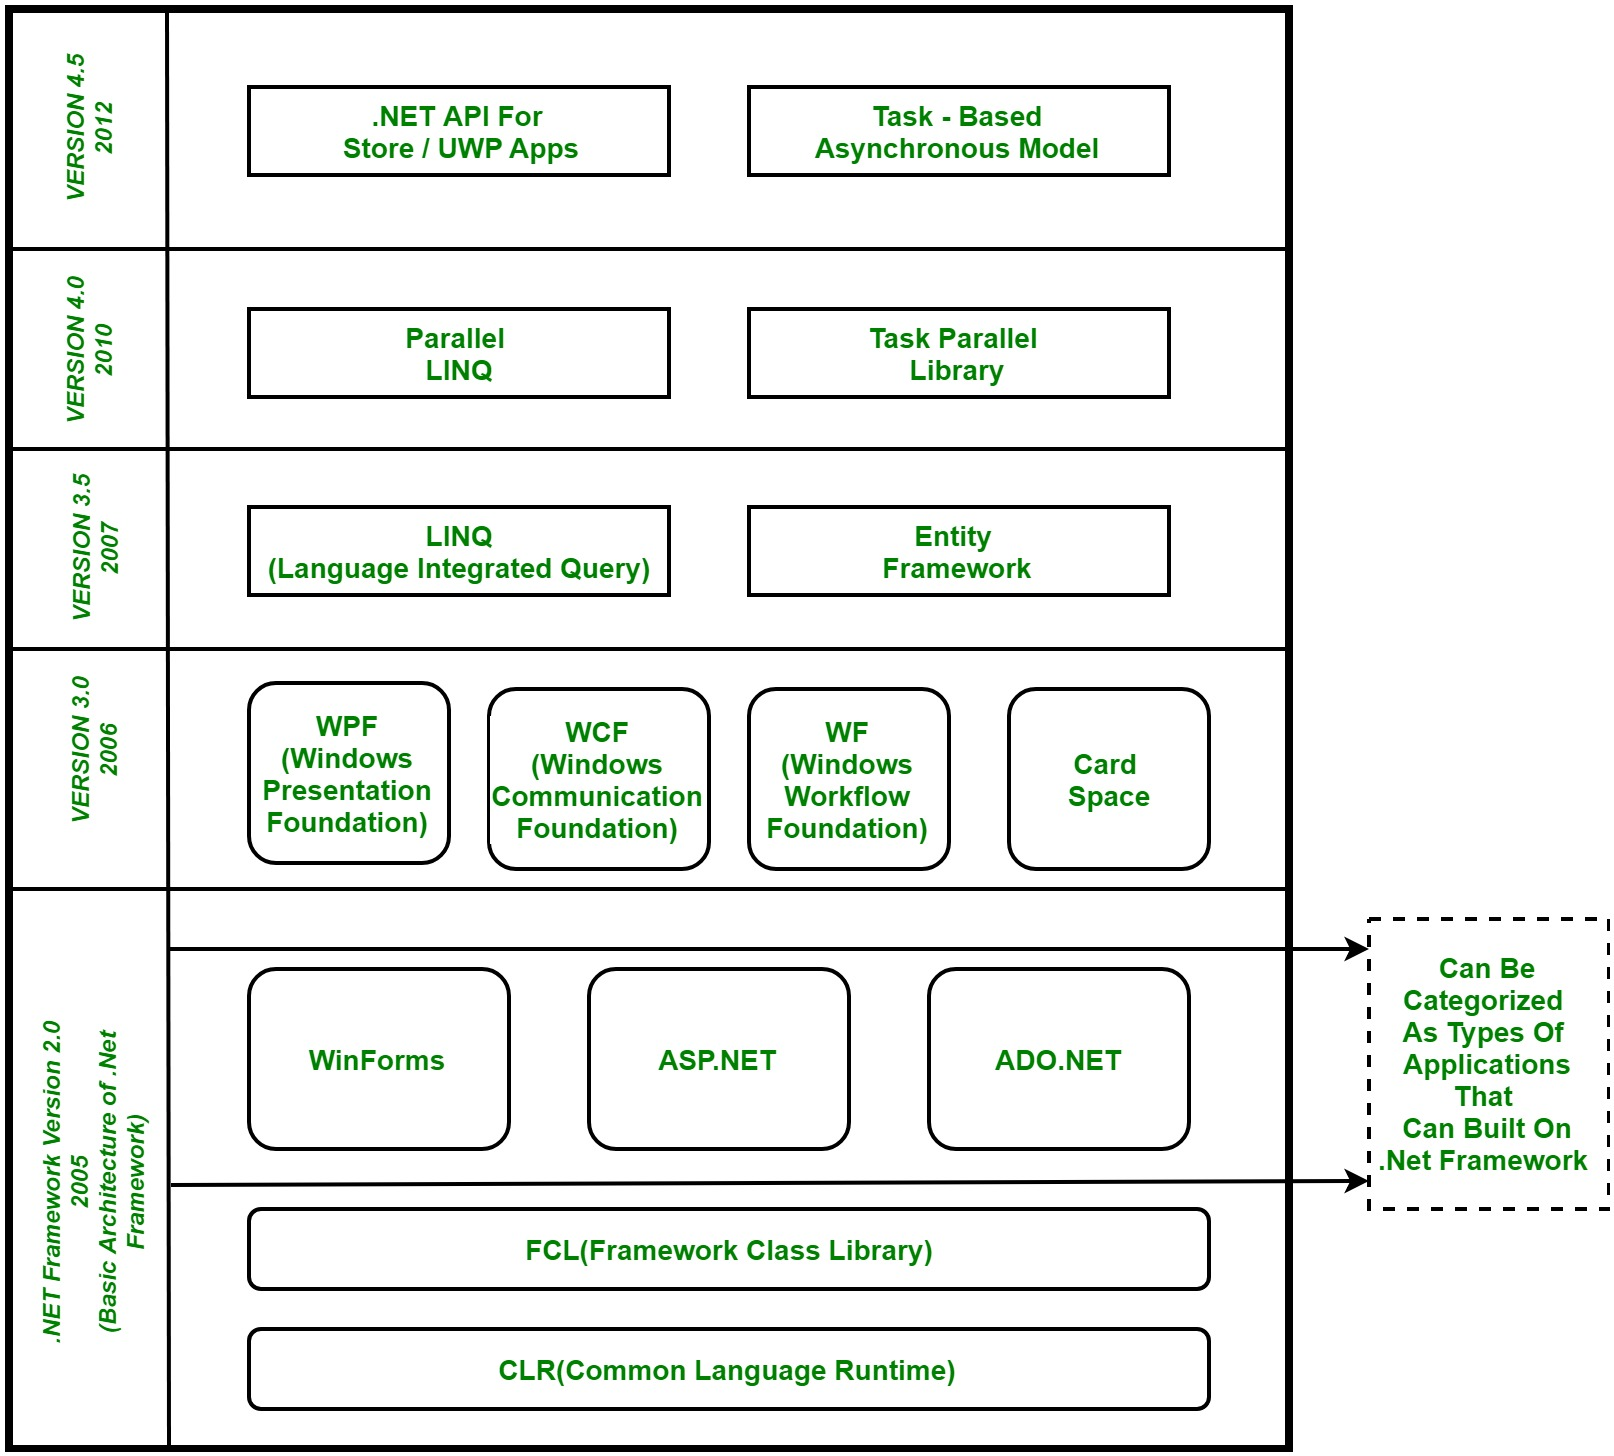
\includegraphics[width=1\textwidth]{Images/net-framework-stack.jpeg}
\caption{\label{fig:netstack}La pila tecnologica dei componenti di \gls{.net} (2005/2012).}
\end{figure}


\subsection{ASP.NET}\label{sec:asp.net}
Una delle principali tecnologie di \gls{.net} è \acrfull{asp.net}, utilizata ampiamente in questo progetto di prova finale. 
\acrshort{asp.net} è un \gls{framework} di sviluppo web, sviluppato da Microsoft, esattamente come il suo `fratello maggiore' \gls{.net}; è stato rilasciato per la prima volta nel gennaio 2002 con la versione 1.0 del \gls{framework} \gls{.net}. Attualmente, la versione più recente è la 4.8.1, rilasciata nel 2022.
Al giorno d'oggi, in un mondo in cui le applicazioni web fanno sempre più parte della nostra vita quotidiana, scegliere il \gls{framework} più adatto è essenziale per sviluppare applicazioni web robuste, scalabili e manutenibili.
\acrshort{asp.net} è un \gls{framework} prominente in quest'ambito, offrendo agli sviluppatori la possibilitò di creare applicazioni web moderne e piene di funzionalità.\newline

Le funzionalità chiave di \acrshort{asp.net} includono:
\begin{itemize}
    \item \acrfull{mvc}: pattern architetturale che facilita la separazione delle responsabilità tra i 3 componenti (modello, vista e controller). Inoltre, il modello \acrshort{mvc} favorisce codice organizzato, modulare e facile da mantenere, contribuendo alla scalabilità dell'applicazione web;
    \item \text{C\#}\footnote{\glsdesc{csharp}}: uno degli aspetti distintivi di \acrshort{asp.net} è la sua integrazione con il linguaggio di programmazione \text{C\#} per la programmazione lato server. Sfruttando le capacità di \text{C\#}, \acrshort{asp.net} introduce principiti fortemente tipati, orientati agli oggetti e un vasto ecosistema di librerie e strumenti per lo sviluppo web, ottenendo un codice più efficiente e mantenibile;
    \item Multi-piattaforma: \acrshort{asp.net} offre ampio supporto per Windows, Linux e macOS, espandendo la portata delle applicazioni web e facilitando l'adozione di pratiche di sviluppo moderne, come le architetture a microservizi e la containerizzazione\footnote{\glsdesc{containerizzazione}};
    \item Supporto \acrfull{ide}\footnote{\glsdesc{IDE}}: lo sviluppo \acrshort{asp.net} è uniformemente integrato con Visual Studio, un potente \acrshort{IDE}, il quale offre una miriade di funzionalità, alcune esclusive per \acrshort{asp.net}.
\end{itemize}

\begin{figure}[H]
\centering
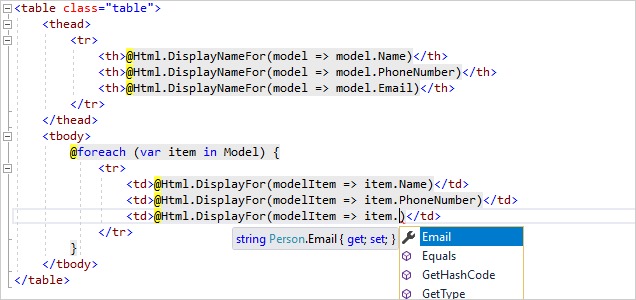
\includegraphics[width=1\textwidth]{Images/aspnet example (razor).png}
\caption{\label{fig:aspnet example}Esempio di una semplice applicazione web  \acrshort{asp.net}.}
\end{figure}

L'utilizzo di \acrshort{asp.net} offre una serie di vantaggi empirici, tra cui:
\begin{itemize}
    \item Scalabilità e alte prestazioni: \acrshort{asp.net} è noto per la sua capacità di gestire carichi elevati e offrire prestazioni eccezionali. Funzionalità come la compilazione `just-in-time'\footnote{\glsdesc{just-in-time}}, la memorizzazione dell'output nella cache e la programmazione asincrona contribuiscono alla scalabilità delle applicazioni web, garantendo un'esperienza d'uso scattante all'utente, anche sotto carichi pesanti;
    \item Sicurezza: funzionalità di priorità nel web development e \acrshort{asp.net} offre un set di funzionalità robusto per affrontare varie problematica di sicurezza, come ad esempio meccanismi di autenticazione integrati, procedure di codifica sicura e protezione contro le vulnerabilità più comuni. Tutto ciò migliora la stabilità complessiva delle applicazioni web di \acrshort{asp.net};
    \item Ecosistema ricco e supporto della comunità: l'ecosistema \acrshort{asp.net} è ricco di librerie, \gls{framework} e estensioni che accelerano e facilitano lo sviluppo. Inoltre, la comunità attiva intorno a \acrshort{asp.net} garantisce un supporto continuo, aggiornamenti frequenti e un'ampia varietà di risorse per gli sviluppatori che cercano di migliorare le proprie competenze i specifici ambiti.
\end{itemize}

\begin{figure}[H]
\centering
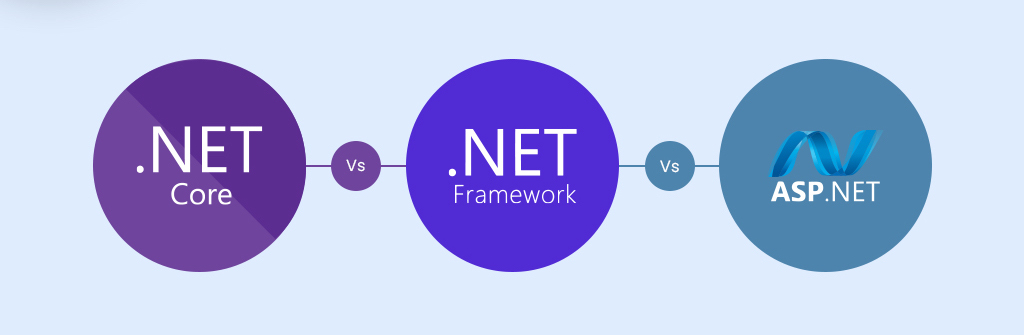
\includegraphics[width=1\textwidth]{Images/net vs.jpg}
\caption{\label{fig:net vs}Le principali tecnologie Microsoft \gls{.net}.}
\end{figure}

Concludendo, \acrshort{asp.net} resta una forza trainante nello sviluppo web, offrendo un \gls{framework} completo e versatile per la loro costruzione. La sua architettura robusta, il supporto per lo sviluppo multi-piattaforma e l'integrazione con potenti strumenti di sviluppo lo rendono una scelta convincente per gli sviluppatori che mirano a fornire soluzioni web di alta qualità, scalabili e sicure.
\begin{figure}[H]
\centering

\includegraphics[width=.5\textwidth]{Images/c-sharp.png}
\caption{\label{fig:c-sharp}Logo di C\#.}
\end{figure}